\documentclass[a4paper,11pt]{article}

%%%%%%%%%%%%%%%%%%%%%%%%%%%%%%%%%%%%%%%%%%%%%%%%%%%%%%%%%%%%%%%%%%%%%%%%
% Paquetes utilizados
%%%%%%%%%%%%%%%%%%%%%%%%%%%%%%%%%%%%%%%%%%%%%%%%%%%%%%%%%%%%%%%%%%%%%%%%

% Graficos complejos
\usepackage{graphicx}
\usepackage{caption}
\usepackage{subcaption}
\usepackage{placeins}

% Soporte para el lenguaje español
\usepackage{textcomp}
\usepackage[utf8]{inputenc}
\usepackage[T1]{fontenc}
\DeclareUnicodeCharacter{B0}{\textdegree}
\DeclareUnicodeCharacter{00A0}{ }
\usepackage[spanish]{babel}

% Codigo fuente embebido
\usepackage{listings}

% PDFs embebidos para el apendice
\usepackage{pdfpages}

% Matematicos
\usepackage{amssymb,amsmath}

% Tablas complejas
\usepackage{multirow}
\usepackage{textcomp}

% Formato de parrafo
\setlength{\parskip}{1ex plus 0.5ex minus 0.2ex}

%%%%%%%%%%%%%%%%%%%%%%%%%%%%%%%%%%%%%%%%%%%%%%%%%%%%%%%%%%%%%%%%%%%%%%%%
% Titulo
%%%%%%%%%%%%%%%%%%%%%%%%%%%%%%%%%%%%%%%%%%%%%%%%%%%%%%%%%%%%%%%%%%%%%%%%

% Titulo principal del documento.
\title{\textbf{Trabajo Practico Promocional: Deteccion de fraude en
telefonía celular con Redes Neuronales}}

% Informacion sobre los autores.
\author{\\
  Daniel Mugica, \textit{P. 87.967}                                \\
  \texttt{fiubadaniel@gmail.com}                                   \\ [2.5ex]
  Sergio Matias Piano, \textit{P. 85.191}                          \\
  \texttt{smpiano@gmail.com}                                       \\ [2.5ex]
                                                                   \\
  \normalsize{1er. Cuatrimestre de 2013}                           \\
  \normalsize{75.23 Inteligencia Artificial}                       \\
  \normalsize{Facultad de Ingenieria, Universidad de Buenos Aires} \\
}
\date{}

%%%%%%%%%%%%%%%%%%%%%%%%%%%%%%%%%%%%%%%%%%%%%%%%%%%%%%%%%%%%%%%%%%%%%%%%
% Documento
%%%%%%%%%%%%%%%%%%%%%%%%%%%%%%%%%%%%%%%%%%%%%%%%%%%%%%%%%%%%%%%%%%%%%%%%

\begin{document}

% ----------------------------------------------------------------------
% Top matter
% ----------------------------------------------------------------------
\thispagestyle{empty}
\maketitle

\begin{abstract}

  Este informe sumariza el desarrollo del trabajo practico 1 de la materia
  Inteligencia Artificial (75.23) dictada en el primer cuatrimestre de
  2013 en la Facultad de Ingenieria de la Universidad de Buenos Aires. El mismo
  consiste en la detección de fraude por telefonía celular a través de la
  utilización de redes neuronales.

\end{abstract}

\clearpage



\section{Introducción}


En el  presente  trabajo  vamos  a  mostrar  una  aplicación  de  las  redes
neuronales  hacia  la  detección  de  comportamientos  fraudulentos  en   la
industria de telefonía celular. Para lograr este  objetivo  vamos  a  buscar
patrones dentro de una actividad en la que pueda existir fraude.


\section{¿Qué es un patrón?}


      Un patrón es una entidad a la que se le puede  dar  un  nombre  y  que
está representada por un conjunto de propiedades medidas  y  las  relaciones
entre ellas, llamado vector de características.
Por  ejemplo,  un  patrón  puede  ser  una  señal  sonora  y  su  vector  de
características el conjunto de coeficientes espectrales extraídos de ella.

      Otro ejemplo podría ser una imagen de una cara humana  de  las  cuales
se extrae el vector de características formado por un  conjunto  de  valores
numéricos calculados a partir de la  misma.  El  reconocimiento  automático,
descripción,  clasificación  y  agrupamiento  de  patrones  son  actividades
importantes en una gran variedad de disciplinas científicas, como  biología,
sicología,  medicina,  visión  por  computador,   inteligencia   artificial,
teledetección, etc.

      En el caso de querer identificar operaciones de fraude podrían  llegar
a  ser  una  transacción  bancaria  en  un  banco   'x'   cuyo   vector   de
características podrían ser todos los datos de las mismas:  montos,  fechas,
personas físicas y/o jurídicas, datos de cuentas,  situación  crediticia  de
las personas, etc.

      Un sistema de reconocimiento de patrones tiene uno de  los  siguientes
objetivos:
      a.- Identificar el patrón  como  miembro  de  una  clase  ya  definida
(clasificación supervisada).
      b.- Asignar el patrón a una clase todavía no  definida  (clasificación
no supervisada,  agrupamiento o clustering).

      Una forma de realizar el reconocimiento de patrones  es  a  través  de
procesamientos por redes neuronales. Podemos ver de cierta forma  que  ambos
objetivos se parecen mucho a lo visto en los  métodos  de  aprendizajes  que
las mismas proveen, por lo cual es una  forma  muy  natural  de  encarar  el
problema.


\section{Redes Neuronales}

Las redes de  neuronas  artificiales  son  un  paradigma  de  aprendizaje  y
procesamiento automático inspirado en la forma en que  funciona  el  sistema
nervioso. Se trata de un sistema de interconexión de  neuronas  en  una  red
que colabora para producir un estímulo de salida.


\begin{figure}[h!]
  \centering
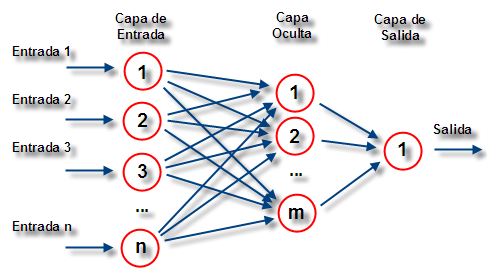
\includegraphics{docs/RedNeuronalArtificial.png}
  \caption{Red Neuronal Artificial}
\end{figure}


\section{Modelo de una Neurona}

\begin{figure}[h!]
  \centering
  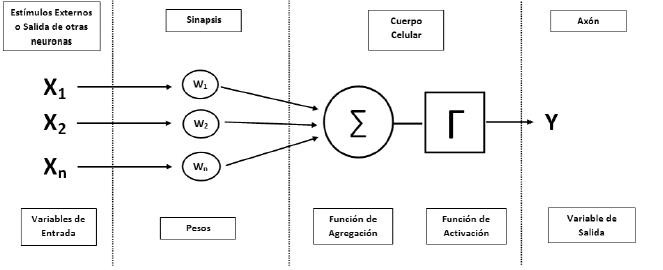
\includegraphics[scale=0.5]{docs/neurona.jpg}
  \caption{Modelo de una neurona arificial tomada de la biológica}
\end{figure}

Una red neuronal se compone de  unidades  llamadas  neuronas.  Cada  neurona
recibe una serie de  entradas  a  través  de  interconexiones  y  emite  una
salida. Esta salida viene dada por tres funciones:

    • Una función  de  propagación,  que  por  lo  general  consiste  en  el
      sumatorio  de  cada  entrada  multiplicada   por   el   peso   de   su
      interconexión. Si  el  peso  es  positivo,  la  conexión  se  denomina
      excitatoria; si es negativo, se denomina inhibitoria.


    • Una función de activación,  que  modifica  a  la  anterior.  Puede  no
      existir,  siendo  en  este  caso  la  salida  la  misma   función   de
      propagación.


    • Una función de transferencia, que se aplica al valor devuelto  por  la
      función de activación. Se utiliza para acotar la salida de la  neurona
      y generalmente viene dada por la interpretación que queramos  darle  a
      dichas salidas. Algunas de las más utilizadas son la función sigmoidea
      (valores en el intervalo [0,1]) y la tangente hiperbólica (valores  en
      el intervalo [-1,1]).


\section{Fraudes en la telefonía celular}

      Cuando las primeras redes móviles de comunicaciones analógicas  fueron
lanzadas al  mercado,  su  debilidad  principal  residía  en  la  seguridad,
particularmente en la falta de encriptación de los datos en los  canales  de
comunicación que permitía la clonación de teléfonos celulares (dos  aparatos
diferentes usando la misma cuenta). A medida que  la  tecnología  evolucionó
de analógica a digital, la naturaleza del fraude ha cambiado haciéndose  más
difícil la clonación, y llevando estas  actividades  hacia  otros  tipos  de
fraude;  sin  embargo,  tampoco   las   redes   digitales   están   libradas
completamente del fraude de clonación.

      Al realizar una llamada de celular se registra que la  misma  se  está
realizando y se produce información referida a este evento. Estos datos  son
comúnmente  llamados  CDR’s  (Call  Detail  Records).  Los  CDR’s  contienen
importante información sobre la  llamada  para  que  luego  ésta  pueda  ser
cobrada a quien corresponda.

       No  obstante  también  pueden  ser  usados  para  detectar  actividad
fraudulenta considerando indicadores de fraude bien  estudiados.  Es  decir,
procesando una cantidad de CDR’s recientes y comparando una función  de  los
diferentes  campos  tales  como  IMSI   (International   Mobile   Subscriber
Identity, que identifica unívocamente un usuario en  una  red  de  telefonía
celular), fecha de la  llamada,  hora  de  la  llamada,  duración,  tipo  de
llamada con un cierto criterio determinado.  Si  esta  función  devuelve  un
valor que se considera fuera de los límites normales, se activa una  alarma,
que debe ser tomada en cuenta por los analistas de fraude para constatar  si
realmente hubo o no actividad de mala fe.

      Para poder procesar estos CDR’s es necesario realizar  previamente  un
proceso conocido en telecomunicaciones como mediación, en el cual se lee  la
información con el formato de registro en el que  vienen  los  CDR’s   y  se
codifica en un nuevo formato  de  registro  entendible  por  el  sistema  de
fraude en este caso.

      Los sistemas existentes de  detección  de  fraude  intentan  consultar
secuencia de CDR’s comparando alguna función de  los  campos  con  criterios
fijos conocidos como Triggers. Un trigger, si es activado, envía una  alarma
que lleva a la investigación por parte de los analistas de fraude.



      Estos sistemas realizan  lo que se conoce como  Análisis  absoluto  de
CDR’s y son buenos para detectar los extremos de la  actividad  fraudulenta.
En cambio, para realizar un análisis diferencial, se monitorean patrones  de
comportamiento  del  teléfono   celular   comparando   sus   más   recientes
actividades con la historia de uso del mismo. Un  cambio  en  el  patrón  de
comportamiento  es  una  característica  sospechosa  de  ser  un   escenario
fraudulento.


A su vez dentro del análisis diferencial hay diferentes enfoques en la
detección de fraude


      • El enfoque por enseñanza: el cual se tipifica por el  uso  de  redes
neuronales supervisadas o herramientas de detección  de  fraude  basadas  en
reglas. A estas herramientas se les presentan casos de fraude  existentes  y
luego tratan de encontrar indicios de fraude basado en lo que han  aprendido
o “se les enseñó”. El enfoque por enseñanza es útil para detectar fraude  de
violación de seguridad.

      • El enfoque por aprendizaje: en el cual generalmente se tipifica  por
el  uso  de  redes  neuronales  no  supervisadas  donde  la  herramienta  de
detección de fraude aprende por sí sola cuál es el  comportamiento  esperado
del usuario. Es muy útil para detectar cambios de comportamiento  y  por  lo
tanto más eficiente en la detección de fraude por  suscripción  y  violación
de seguridad.


\textit{Enfoque por enseñanza}

      En este enfoque, es necesario tener ejemplos reales de  fraude.  Estos
ejemplos son usados para “enseñar” a la  herramienta  qué  es  lo  que  debe
buscar. En el caso  de  un  sistema  basado  en  reglas,  los  ejemplos  son
analizados por sus componentes de fraude que luego  se  traducen  en  reglas
que utilizan  umbrales  o  medidas  relativas.  En  el  caso  de  las  redes
neuronales supervisadas se usan los ejemplos de fraude  y  los  ejemplos  de
usuarios  no  fraudulentos  para   enseñarle   a   la   herramienta   cuáles
comportamientos son buenos y cuáles no lo son. Ambos tipos  de  herramientas
deberían  identificar  comportamientos  de  alguna  manera  similar  a   los
ejemplos de fraude usados o  a  los  ejemplos  de  buen  comportamiento;  si
identifican algún  comportamiento  como  “parecido”  al  de  un  ejemplo  de
fraude, deben emitir una alarma.

\textit{Enfoque por aprendizaje}

      En este enfoque, la herramienta aprenderá el comportamiento típico  de
un usuario y emitirá una alarma cuando  este  comportamiento  haya  cambiado
sensiblemente.  La  habilidad  de  la   herramienta   para   monitorear   el
comportamiento de los usuarios la hace muy útil  para  detectar  fraudes  de
los que no se sabe nada como así todos los casos de fraude por  suscripción,
que resultan en cambios de  comportamiento.  Si  se  sabe  poco  acerca  del
fraude existente en el sistema, esta  es  una  buena  forma  de  trabajar  y
obtener buenos ejemplos de  comportamiento  fraudulento;  sin  embargo,  hay
algunos puntos importantes a tener en cuenta cuando se utiliza este  enfoque
entre los cuales se puede destacar que no

es posible enseñarle a esta herramienta qué buscar y si  los  parámetros  de
evolución no se  configuran  correctamente,  puede  llegar  a  fallar  y  no
detectar cambios de comportamiento que lancen las alarmas correspondientes.
      Un modelo de red neuronal muy utilizado en la detección de fraudes  es
el conocido como Self-Organizing Map.



\section{Self-Organizing Map}

      Los Self-Organizing Map ó SOM, también llamados redes de Kohonen, son
un tipo de red neuronal no supervisada, competitiva,  distribuida  de  forma
regular en una  rejilla  de,  normalmente,  dos  dimensiones,  cuyo  fin  es
descubrir la estructura subyacente de los datos introducidos en ella.  A  lo
largo del entrenamiento de la red, los vectores de  datos  son  introducidos
en cada neurona y se comparan con el vector de peso característico  de  cada
neurona. La neurona que presenta menor diferencia entre su vector de peso  y
el vector de datos es la neurona ganadora  (o BMU)  y  ella  y  sus  vecinas
verán modificados sus vectores de pesos.
      Las neuronas de la SOM están distribuidas en forma de rejilla de una o
dos dimensiones, dependiendo de la manera en que se quieran  visualizar  los
datos. Las más comunes son las de dos dimensiones. Rejillas  de  dimensiones
superiores son posibles, aunque son más difíciles de interpretar.
En las SOM de dos dimensiones, se pueden distinguir dos tipos de rejillas:
    • Rejilla hexagonal: en ella cada neurona tiene  seis  vecinos  (excepto
      los extremos).
    • Rejilla rectangular: cada neurona tiene cuatro vecinos.


\begin{figure}[h!]
  \centering
  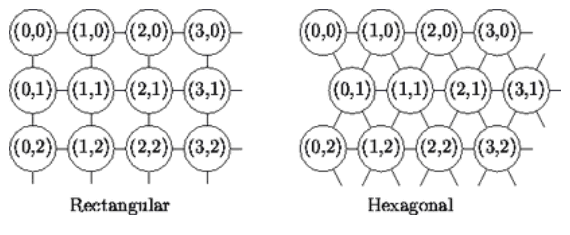
\includegraphics[scale=0.7]{docs/rejillas.png}
  \caption{Modelos de las rejillas}
\end{figure}

      Cada neurona de  la  red  tiene  asociado  un vector  de  pesos (o  de
prototipo) de la misma dimesión  que  los  datos  de  entrada.  Éste  sería
el espacio de entrada de la red, mientras que el espacio de salida sería  la
posición en el mapa de cada neurona.
      Las neuronas mantienen con sus  vecinas relaciones  de  vecindad,  las
cuales son claves para conformar el mapa durante la etapa de  entrenamiento.
Esta relación viene dada por una función.
Entrenamiento de la red:

\begin{enumerate}

   \item Inicializar pesos. Asignar a los pesos valores pequeños aleatorios.

   \item Presentar una nueva entrada (El conjunto de  aprendizaje  se  presenta
     cíclicamente hasta llegar a la convergencia de la red. Actualizar \textit{alfa}).

   \item Propagar el patrón de entrada hasta la capa  de  competición.  Obtener
      los valores de salida de las células de dicha capa.

   \item Seleccionar la célula ganadora C cuya salida sea menor.

   \item Actualizar las conexiones entre la capa de entrada y la célula C,  así
      como las de su vecindad, según su grado de vecindad.

   \item Si \textit{alfa} por encima de cierto umbral volver al paso 2, en  caso  contrario
      FIN.

\end{enumerate}
\end{document}
